\subsection{UC8: Condivisione dei grafici}
\hypertarget{UC8}{}
\begin{figure} [H]
	\centering
	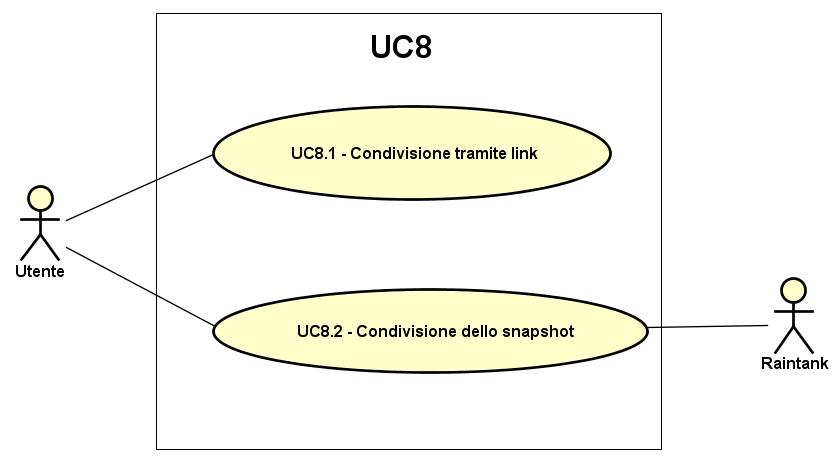
\includegraphics[scale=0.45]{Img/UC8}
	\caption{UC8 - Condivisione dei grafici}\label{}
\end{figure}
\begin{itemize}
	\item \textbf{Attori}: Utente;
	\item \textbf{Attori secondari}: Raintank;
	\item \textbf{Scopo e descrizione}: l'utente può condividere i grafici presenti nella dashboard;
	\item \textbf{Precondizione}: il sistema mette a disposizione diversi modi per effettuare la condivisione dei grafici;
	\item \textbf{Scenario principale}:
	\begin{itemize}
		\item Condivisione tramite link (UC8.1);	
		\item Condivisione dello snapshot (UC8.2).
	\end{itemize}
	\item \textbf{Postcondizione}: il grafico è stato condiviso nel modo scelto dall'utente.
	
\end{itemize}

\subsection{UC8.1: Condivisione tramite link}
\hypertarget{UC8.1}{}
\begin{figure} [H]
	\centering
	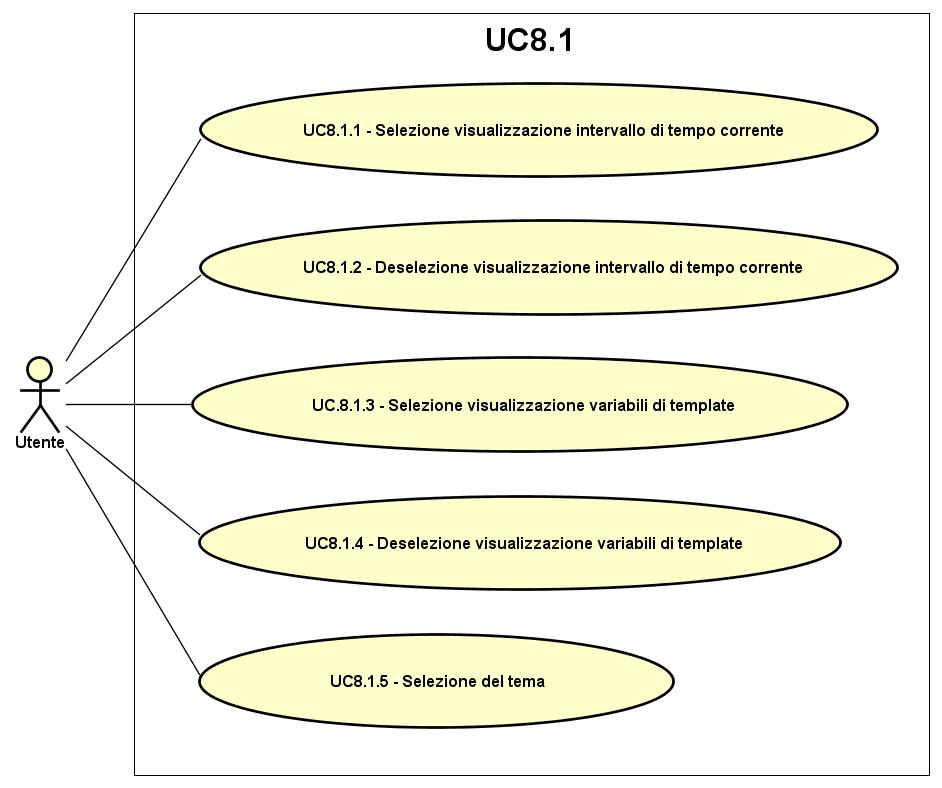
\includegraphics[scale=0.45]{Img/UC8-1}
	\caption{UC8.1 - Condivisione tramite link}\label{}
\end{figure}
\begin{itemize}
	\item \textbf{Attori}: Utente;
	\item \textbf{Scopo e descrizione}: l'attore visualizza un link diretto alla dashboard o ad un panel, generato sulla base delle opzioni scelte;
	\item \textbf{Precondizione}: il sistema permette la visualizzazione di link per la condivisione di dashboard e panel e ne permette all'attore di selezionare varie opzioni;
	\item \textbf{Scenario principale}:
	\begin{itemize}
		\item Selezione visualizzazione intervallo di tempo corrente (UC8.1.1);
		\item Deselezione visualizzazione intervallo di tempo corrente (UC8.1.2);
		\item Selezione visualizzazione variabili di template (8.1.3);
		\item Deselezione visualizzazione variabili di template (8.1.4);
		\item Selezione del tema (UC8.1.5).
	\end{itemize}
	\item \textbf{Postcondizione}: Viene mostrato il link per la condivisione del grafico.
\end{itemize}

\subsection{UC8.1.1: Selezione visualizzazione intervallo di tempo corrente}
\hypertarget{UC8.1.1}{}
\begin{itemize}
	\item \textbf{Attori}: Utente;
	\item \textbf{Scopo e descrizione}: l'attore seleziona la visualizzazione dell'intervallo di tempo in cui sono stati raccolti i dati presenti nel grafico;
	\item \textbf{Precondizione}: il sistema permettere di selezionare la visualizzazione dell'intervallo di tempo in un grafico;
	\item \textbf{Scenario principale:} l'attore seleziona l'opzione che visualizza l'intervallo di tempo corrente in un grafico;
	\item \textbf{Postcondizione}: l'intervallo di tempo in cui sono stati raccolti i dati presenti viene visualizzato nel grafico.
\end{itemize}

\subsection{UC8.1.2: Deselezione visualizzazione intervallo di tempo corrente}
\hypertarget{UC8.1.2}{}
\begin{itemize}
	\item \textbf{Attori}: Utente;
	\item \textbf{Scopo e descrizione}: l'attore deseleziona la visualizzazione dell'intervallo di tempo in cui sono stati raccolti i dati presenti nel grafico;
	\item \textbf{Precondizione}: il sistema permettere di deselezionare la visualizzazione dell'intervallo di tempo in un grafico;
	\item \textbf{Scenario principale:} l'attore deseleziona l'opzione che visualizza l'intervallo di tempo corrente in un grafico;
	\item \textbf{Postcondizione}: l'intervallo di tempo in cui sono stati raccolti i dati presenti non viene visualizzato nel grafico.
\end{itemize}

\subsection{UC8.1.3: Selezione visualizzazione variabili di template}
\hypertarget{UC8.1.3}{}
\begin{itemize}
	\item \textbf{Attori}: Utente;
	\item \textbf{Scopo e descrizione}: l'attore seleziona la visualizzazione delle variabili di template nel grafico;
	\item \textbf{Precondizione}: il sistema permette di selezionare la visualizzazione delle variabili di template in un grafico;
	\item \textbf{Scenario principale:} l'attore seleziona l'opzione che visualizza le variabili di template in un grafico;
	\item \textbf{Postcondizione}: le variabili di template vengono visualizzate nel grafico.
\end{itemize}

\subsection{UC8.1.4: Deselezione visualizzazione variabili di template}
\hypertarget{UC8.1.4}{}
\begin{itemize}
	\item \textbf{Attori}: Utente;
	\item \textbf{Scopo e descrizione}: l'attore deseleziona la visualizzazione delle variabili di template nel grafico;
	\item \textbf{Precondizione}: il sistema permette di deselezionare la visualizzazione delle variabili di template in un grafico;
	\item \textbf{Scenario principale:} l'attore deseleziona l'opzione che visualizza le variabili di template in un grafico;
	\item \textbf{Postcondizione}: le variabili di template non vengono visualizzate nel grafico.
\end{itemize}

\subsection{UC8.1.5: Selezione del tema}
\hypertarget{UC8.1.5}{}
\begin{itemize}
	\item \textbf{Attori}: Utente;
	\item \textbf{Scopo e descrizione}: l'attore seleziona i colori di sfondo del grafico; 
	\item \textbf{Precondizione}: il sistema permette la selezione di temi tra quelli predefiniti;
	\item \textbf{Scenario principale:} l'attore seleziona il tema di un grafico;
	\item \textbf{Postcondizione}: il tema del grafico viene selezionato.
\end{itemize}

\subsection{UC8.2: Condivisione dello snapshot}
\hypertarget{UC8.2}{}
\begin{figure} [H]
	\centering
	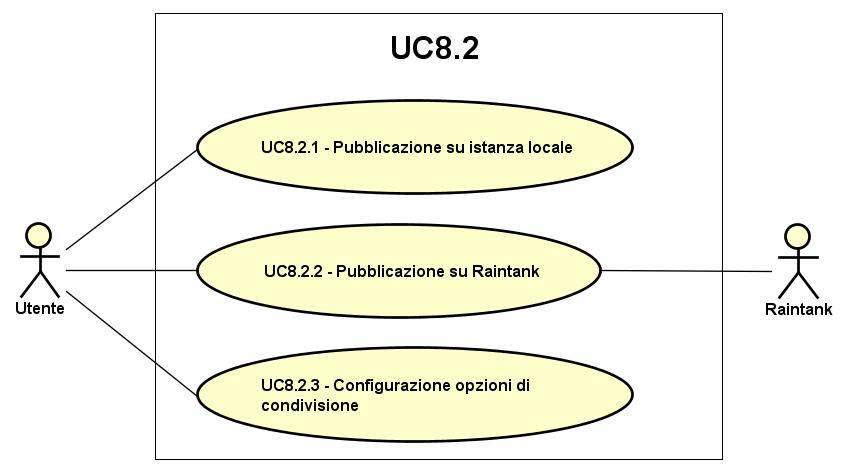
\includegraphics[scale=0.45]{Img/UC8-2}
	\caption{UC8.2 - Condivisione dello snapshot}\label{}
\end{figure}
\begin{itemize}
	\item \textbf{Attori}: Utente;
	\item \textbf{Attori secondari}: Raintank;
	\item \textbf{Scopo e descrizione}: l'utente condivide lo snapshot della dashboard o di un panel;
	\item \textbf{Precondizione}: il sistema permette la condivisione di snapshot;
	\item \textbf{Scenario principale}:
	\begin{itemize}
		\item Pubblicazione su istanza locale (UC8.4.1);
		\item Pubblicazione su Raintank (UC8.4.2);
		\item Configurazione opzioni di visualizzazione (UC8.4.3).
	\end{itemize}
	\item \textbf{Postcondizione}: lo snapshot con le relative opzioni di visualizzazione è stato condiviso dall'utente.
\end{itemize}

\subsection{UC8.2.1: Pubblicazione su istanza locale}
\hypertarget{UC8.2.1}{}
\begin{itemize}
	\item \textbf{Attori}: Utente;
	\item \textbf{Scopo e descrizione}: l'attore pubblica lo snapshot della dashboard o di un panel sulla sua istanza locale;
	\item \textbf{Precondizione}: il sistema permette la pubblicazione di snapshot sull'istanza di un utente;
	\item \textbf{Scenario principale:} l'attore pubblica un grafico sulla sua istanza locale;
	\item \textbf{Postcondizione}: lo snapshot è stato pubblicato sull'istanza.
\end{itemize}

\subsection{UC8.2.2: Pubblicazione su Raintank}
\hypertarget{UC8.2.2}{}
\begin{itemize}
	\item \textbf{Attori}: Utente;
	\item \textbf{Attori secondari}: Raintank;
	\item \textbf{Scopo e descrizione}: l'utente pubblica lo snapshot della dashboard o di un panel sulla piattaforma Raintank;
	\item \textbf{Precondizione}: il sistema permette la pubblicazione di snapshot su Raintank;
	\item \textbf{Scenario principale:} l'utente pubblica un grafico su Raintank;
	\item \textbf{Postcondizione}: lo snapshot è stato pubblicato su Raintank.
\end{itemize}

\subsection{UC8.2.3: Configurazione opzioni di pubblicazione}
\hypertarget{UC8.2.3}{}
\begin{figure} [H]
	\centering
	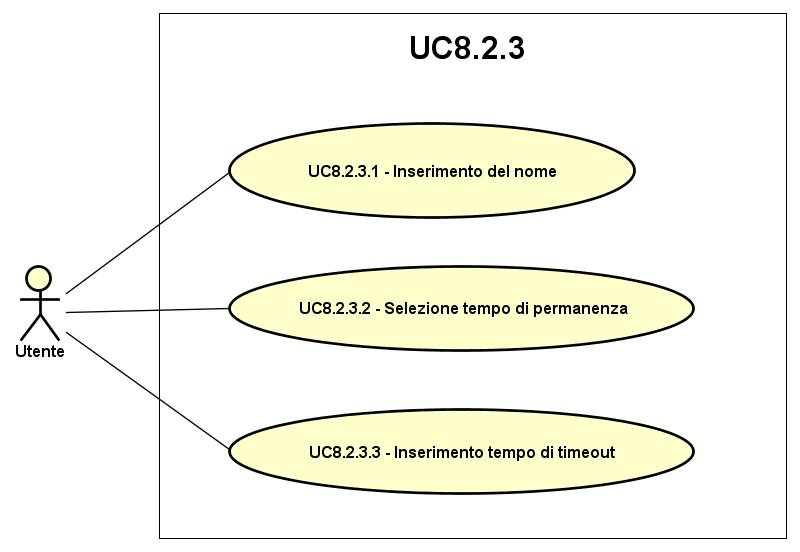
\includegraphics[scale=0.45]{Img/UC8-2-3}
	\caption{UC8.2.3 - Configurazione opzioni di pubblicazione}\label{}
\end{figure}
\begin{itemize}
	\item \textbf{Attori}: Utente;
	\item \textbf{Scopo e descrizione}: l'attore configura le opzioni per la pubblicazione dello snapshot della dashboard o di un panel;
	\item \textbf{Precondizione}: il sistema permette di configurare le opzioni per la pubblicazione di snapshot;
	\item \textbf{Scenario principale}:
	\begin{itemize}
		\item Inserimento del nome (UC8.2.3.1);
		\item Selezione tempo di permanenza (UC8.2.3.2);
		\item Inserimento tempo per timeout (UC8.2.3.3).
	\end{itemize}
	\item \textbf{Postcondizione}: le opzioni per la pubblicazione dello snapshot sono state configurate.
\end{itemize}

\subsection{UC8.2.3.1: Inserimento del nome}
\hypertarget{UC8.2.3.1}{}
\begin{itemize}
	\item \textbf{Attori}: Utente;
	\item \textbf{Scopo e descrizione}: l'attore inserisce il nome dello snapshot;
	\item \textbf{Precondizione}: il sistema permette l'inserimento del nome di uno snapshot;
	\item \textbf{Scenario principale:} l'utente inserisce il nome di uno snapshot;
	\item \textbf{Postcondizione}: il nome dello snapshot è stato inserito.
\end{itemize}

\subsection{UC8.2.3.2: Selezione tempo di permanenza}
\hypertarget{UC8.2.3.2}{}
\begin{itemize}
	\item \textbf{Attori}: Utente;
	\item \textbf{Scopo e descrizione}: l'attore seleziona il tempo di permanenza di uno snapshot dal momento della sua pubblicazione;
	\item \textbf{Precondizione}: il sistema permette di selezionare il tempo di permanenza di uno snapshot tra le opzioni predefinite;
	\item \textbf{Scenario principale:} l'utente seleziona il tempo di permanenza di uno snapshot;
	\item \textbf{Postcondizione}: il tempo di permanenza dello snapshot è stato selezionato.
\end{itemize}

\subsection{UC8.2.3.3: Inserimento tempo di timeout}
\hypertarget{UC8.2.3.3}{}
\begin{itemize}
	\item \textbf{Attori}: Utente;
	\item \textbf{Scopo e descrizione}: l'attore inserisce il tempo(in secondi) massimo per il caricamento dei dati nello snapshot;
	\item \textbf{Precondizione}: il sistema permette l'inserimento del tempo massimo per il caricamento dei dati di uno snapshot;
	\item \textbf{Scenario principale:} l'utente inserisce il tempo di timeout di uno snapshot;
	\item \textbf{Postcondizione}: il tempo di timeout è stato inserito.
\end{itemize}

\subsection{UC9: Condivisione di panel}
\hypertarget{UC9}{}
\begin{figure} [H]
	\centering
	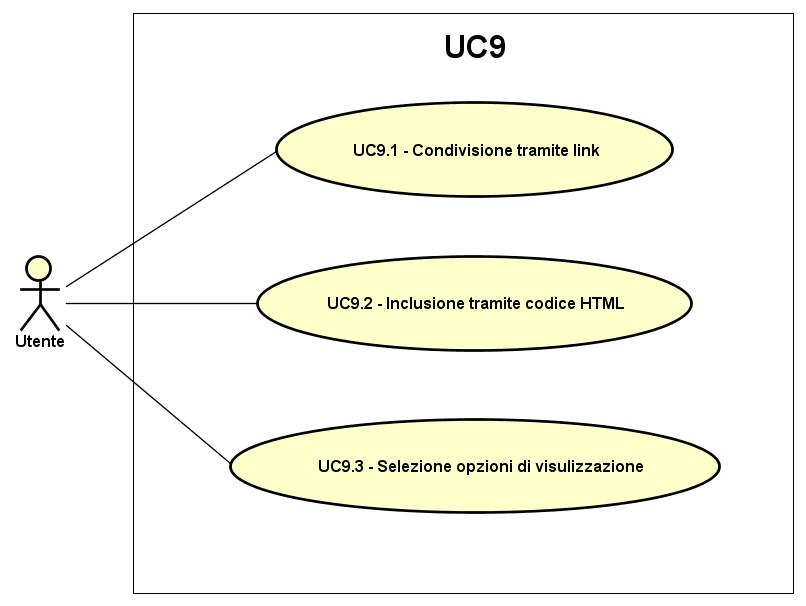
\includegraphics[scale=0.45]{Img/UC9}
	\caption{UC9 - Condivisione di panel}\label{}
\end{figure}
\begin{itemize}
	\item \textbf{Attori}: Utente;
	\item \textbf{Scopo e descrizione}: l'attore può condividere una panel in diversi modi;
	\item \textbf{Precondizione}: il sistema permette la condivisione di panel;
	\item \textbf{Scenario principale}: 
	\begin{itemize}
		\item Inclusione tramite codice HTML (UC9.1);
	\end{itemize}
	\item \textbf{Postcondizione}: viene condiviso il panel.
\end{itemize}


\subsection{UC9.1: Inclusione tramite codice HTML}
\hypertarget{UC9.1}{}
\begin{figure} [H]
	\centering
	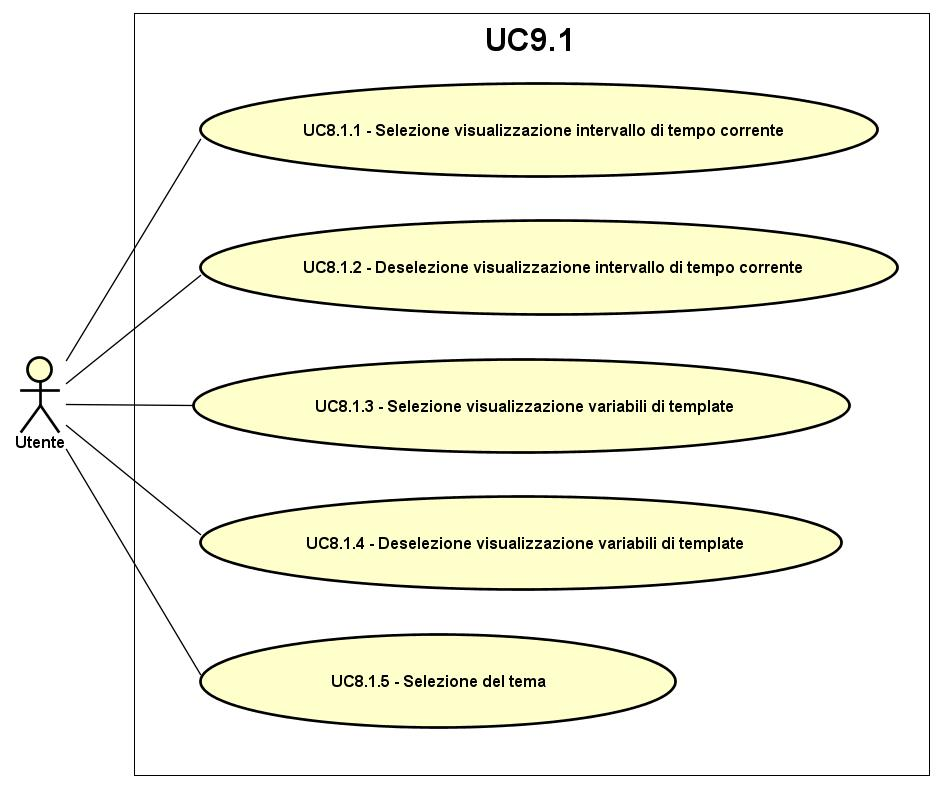
\includegraphics[scale=0.45]{Img/UC9-1}
	\caption{UC9.1 - Inclusione tramite codice HTML}\label{}
\end{figure}
\begin{itemize}
	\item \textbf{Attori}: Utente;
	\item \textbf{Scopo e descrizione}: l'attore visualizza il codice \gl{HTML} per includere un panel in una pagina web, generato sulla base delle opzioni selezionate;
	\item \textbf{Precondizione}: il sistema permette la visualizzazione del codice HTML per l'inclusione di panel, che viene generato sulla base di opzioni che possono essere selezionate dall'attore;
	\item \textbf{Scenario principale}:
	\begin{itemize}
		\item Selezione visualizzazione intervallo di tempo corrente (UC9.1.1);
		\item Deselezione visualizzazione intervallo di tempo corrente (UC9.1.2);
		\item Selezione visualizzazione variabili di template (9.1.3);
		\item Deselezione visualizzazione variabili di template (9.1.4);
		\item Selezione del tema (UC9.1.5).
	\end{itemize}
	\item \textbf{Postcondizione}: viene mostrato il codice HTML per l'inclusione del panel.
\end{itemize}

\subsection{UC9.1.1: Selezione visualizzazione intervallo di tempo corrente}
\hypertarget{UC9.1.1}{}
\begin{itemize}
	\item \textbf{Attori}: Utente;
	\item \textbf{Scopo e descrizione}: l'attore seleziona la visualizzazione dell'intervallo di tempo in cui sono stati raccolti i dati presenti nel grafico;
	\item \textbf{Precondizione}: il sistema permettere di selezionare la visualizzazione dell'intervallo di tempo in un grafico;
	\item \textbf{Scenario principale:} l'attore seleziona l'opzione che visualizza l'intervallo di tempo corrente in un grafico;
	\item \textbf{Postcondizione}: l'intervallo di tempo in cui sono stati raccolti i dati presenti viene visualizzato nel grafico.
\end{itemize}

\subsection{UC9.1.2: Deselezione visualizzazione intervallo di tempo corrente}
\hypertarget{UC9.1.2}{}
\begin{itemize}
	\item \textbf{Attori}: Utente;
	\item \textbf{Scopo e descrizione}: l'attore deseleziona la visualizzazione dell'intervallo di tempo in cui sono stati raccolti i dati presenti nel grafico;
	\item \textbf{Precondizione}: il sistema permettere di deselezionare la visualizzazione dell'intervallo di tempo in un grafico;
	\item \textbf{Scenario principale:} l'attore deseleziona l'opzione che visualizza l'intervallo di tempo corrente in un grafico;
	\item \textbf{Postcondizione}: l'intervallo di tempo in cui sono stati raccolti i dati presenti non viene visualizzato nel grafico.
\end{itemize}

\subsection{UC9.1.3: Selezione visualizzazione variabili di template}
\hypertarget{UC8.1.3}{}
\begin{itemize}
	\item \textbf{Attori}: Utente;
	\item \textbf{Scopo e descrizione}: l'attore seleziona la visualizzazione delle variabili di template nel grafico;
	\item \textbf{Precondizione}: il sistema permette di selezionare la visualizzazione delle variabili di template in un grafico;
	\item \textbf{Scenario principale:} l'attore seleziona l'opzione che visualizza le variabili di template in un grafico;
	\item \textbf{Postcondizione}: le variabili di template vengono visualizzate nel grafico.
\end{itemize}

\subsection{UC9.1.4: Deselezione visualizzazione variabili di template}
\hypertarget{UC8.1.4}{}
\begin{itemize}
	\item \textbf{Attori}: Utente;
	\item \textbf{Scopo e descrizione}: l'attore deseleziona la visualizzazione delle variabili di template nel grafico;
	\item \textbf{Precondizione}: il sistema permette di deselezionare la visualizzazione delle variabili di template in un grafico;
	\item \textbf{Scenario principale:} l'attore deseleziona l'opzione che visualizza le variabili di template in un grafico;
	\item \textbf{Postcondizione}: le variabili di template non vengono visualizzate nel grafico.
\end{itemize}

\subsection{UC9.1.5: Selezione del tema}
\hypertarget{UC8.1.5}{}
\begin{itemize}
	\item \textbf{Attori}: Utente;
	\item \textbf{Scopo e descrizione}: l'attore seleziona i colori di sfondo del grafico; 
	\item \textbf{Precondizione}: il sistema permette la selezione di temi tra quelli predefiniti;
	\item \textbf{Scenario principale:} l'attore seleziona il tema di un grafico;
	\item \textbf{Postcondizione}: il tema del grafico viene selezionato.
\end{itemize}

\subsection{UC10: Condivisione di dashboard}
\hypertarget{UC10}{}
\begin{figure} [H]
	\centering
	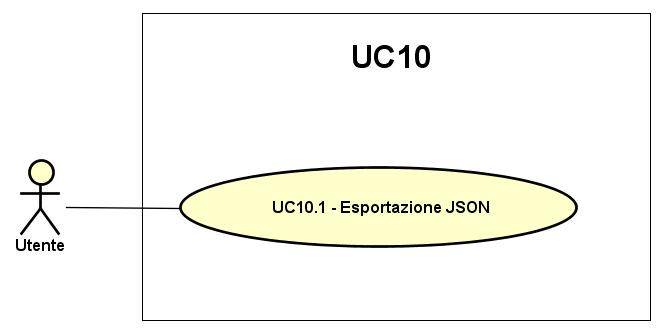
\includegraphics[scale=0.5]{Img/UC10}
	\caption{UC10 - Condivisione di dashboard}\label{}
\end{figure}
\begin{itemize}
	\item \textbf{Attori}: Utente;
	\item \textbf{Scopo e descrizione}: l'attore può condividere una dashboard in diversi modi;
	\item \textbf{Precondizione}: il sistema permette la condivisione di dashboard;
	\item \textbf{Scenario principale}: 
	\begin{itemize}
		\item Esportazione del JSON (UC10.1);
	\end{itemize}
	\item \textbf{Postcondizione}: viene condivisa la dashboard.
\end{itemize}

\subsection{UC10.1: Esportazione JSON}
\hypertarget{UC10.1}{}
\begin{figure} [H]
	\centering
	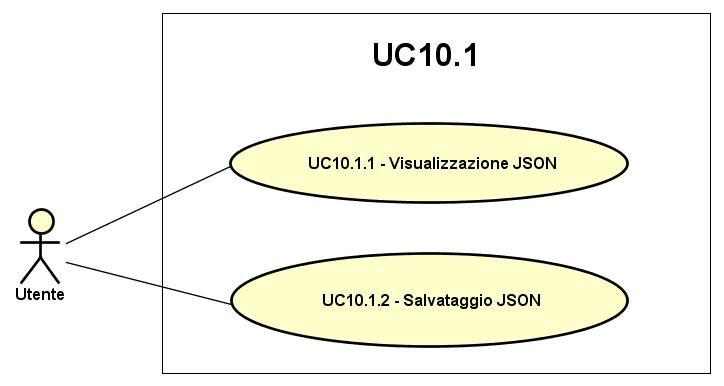
\includegraphics[scale=0.5]{Img/UC10-1}
	\caption{UC10.1 - Esportazione JSON}\label{}
\end{figure}
\begin{itemize}
	\item \textbf{Attori}: Utente;
	\item \textbf{Scopo e descrizione}: l'attore può esportare la struttura di una dashboard definita in un file JSON;
	\item \textbf{Precondizione}: il sistema permette l'esportazione della struttura di una dashboard;
	\item \textbf{Scenario principale}: 
	\begin{itemize}
		\item Visualizzazione del JSON (UC10.1.1);
		\item Salvataggio del JSON (UC10.1.2);
	\end{itemize}
	\item \textbf{Postcondizione}: viene esportato il JSON con la definizione della dashboard.
\end{itemize}

\subsection{UC10.1.1: Visualizzazione JSON}
\hypertarget{UC10.1.1}{}
\begin{itemize}
	\item \textbf{Attori}: Utente;
	\item \textbf{Scopo e descrizione}: l'attore può visualizzare il codice JSON con la struttura di una dashboard;
	\item \textbf{Precondizione}: il sistema permette la visualizzazione della struttura di una dashboard;
	\item \textbf{Scenario principale}: l'attore visualizza la definizione di una dashboard tramite codice JSON;
	\item \textbf{Postcondizione}: viene mostrato il JSON con la definizione della dashboard.
\end{itemize}

\subsection{UC10.1.2: Salvataggio JSON}
\hypertarget{UC10.1.2}{}
\begin{itemize}
	\item \textbf{Attori}: Utente;
	\item \textbf{Scopo e descrizione}: l'attore può salvare localmente il file JSON con la struttura di una dashboard;
	\item \textbf{Precondizione}: il sistema permette il salvataggio della struttura di una dashboard;
	\item \textbf{Scenario principale}: l'attore scarica la definizione di una dashboard tramite un file JSON;
	\item \textbf{Postcondizione}: viene salvato in locale il JSON con la definizione della dashboard.
\end{itemize}

\subsection{UC11: Caricamento di un file non valido}
\hypertarget{UC11}{}
\begin{itemize}
	\item \textbf{Attori}: Utente;
	\item \textbf{Scopo e descrizione}: l'attore tenta di caricare un file dal contenuto non valido o dal formato non valido;
	\item \textbf{Precondizione}: il sistema permette la rilevazione di errori durante il caricamento di un file;
	\item \textbf{Scenario principale}: l'attore tenta di caricare un file che non è valido;
	\item \textbf{Postcondizione}: viene mostrato un messaggio d'errore, il sistema rimane nello stato precedente all'azione.
\end{itemize}


\pagebreak




